\documentclass[conference]{IEEEtran}
\IEEEoverridecommandlockouts

% Packages
\usepackage{cite}
\usepackage{amsmath,amssymb,amsfonts}
\usepackage[dvipsnames]{xcolor}
\usepackage{graphicx}
\usepackage{textcomp}
\usepackage{listings}
\usepackage{subcaption}
\usepackage{multirow}
\usepackage{algorithm}
\usepackage{algpseudocode}
\usepackage{algorithmicx}
\usepackage{todonotes}
\usepackage{url}
\usepackage{caption}  
\usepackage{tcolorbox}
\usepackage{hyperref}

\hypersetup{hidelinks}
\newcommand{\algorithmautorefname}{Algorithm}
\captionsetup[algorithm]{name=Alg.} 

\tcbuselibrary{listingsutf8}
\newtcbox{\redbox}[1][]{
  on line, 
  boxsep=1pt, 
  left=1pt, 
  right=1pt, 
  top=1pt, 
  bottom=1pt, 
  colframe=red!75!black, 
  colback=red!10, 
  boxrule=0.5pt, 
  rounded corners,
  #1
}

\algrenewcommand\algorithmicindent{0.8em} 



\begin{document}

\title{Algorithm Selection and Auto-Tuning in AutoPas}

\author{
    \IEEEauthorblockN{ Manuel Lerchner}
    \IEEEauthorblockA{
        \textit{Technical University of Munich}\\
        Munich, Germany}
}

\maketitle

\begin{abstract}
    Molecular dynamics (MD) simulations face significant computational challenges that require highly optimized simulation engines to deal with the enormous number of particles present in modern simulations. Naturally researchers have put a lot of effort into developing algorithms and frameworks that can efficiently simulate these systems. This paper examines the auto-tuning capabilities of AutoPas, a modern MD framework, and provides a comparative analysis with other prominent MD engines such as GROMACS and LAMMPS. We analyze the approaches to static and dynamic optimization and evaluate their effectiveness in various simulation scenarios. Furthermore, we investigate a possible improvement to the auto-tuning capabilities of AutoPas by introducing an early stopping mechanism to reduce the overhead the parameter space exploration.
    \todo{conclusion}
\end{abstract}

\begin{IEEEkeywords}
    molecular dynamics, auto-tuning, algorithm selection, performance optimization, GROMACS, LAMMPS
\end{IEEEkeywords}

\section{Introduction}

Molecular dynamics simulations represent a computational cornerstone in various scientific fields, from materials science to biochemistry. To deliver accurate results, these simulations typically make use of complex, and computationally intensive interaction-models acting on enourmous number of particles. For simulation engines to be practical, they must be highly optimized to handle the computational load efficiently and utilize available resources effectively.

Prominent optimization techniques used in modern molecular dynamics (MD) engines fall into two main categories: static and dynamic optimization. Static optimizations rely on predefined configurations and performance models, often fine-tuned for specific hardware architectures. These optimizations include strategies like memory layout optimization, vectorization, and architecture-specific instruction use (e.g., SIMD) \todo{Efficient Computation and Optimization Techniques for Molecular Dynamics Simulations, or similar}.

Modern compiler frameworks such as Kokkos and SYCL further abstract hardware-specific optimizations, enabling more portable code across different hardware platforms (e.g., GPUs, CPUs). Kokkos provides a performance-portable parallel programming model that supports diverse high-performance computing environments, while SYCL, a standard by the Khronos Group, facilitates single-source C++ for heterogeneous platform \todo{The Kokkos EcoSystem: Comprehensive Performance Portability for High-Performance Computing; SYCL specifications or Khronos Group publications}.

In contrast, dynamic optimizations adjust parameters based on the current simulation state and the actual hardware performance. Unlike static optimizations, which are set before the simulation begins, dynamic optimizations allow for adjustments throughout the simulation. This approach enables MD engines to periodically measure and respond to actual performance, optimizing parameters like load balancing, cache locality, and communication patterns to improve efficiency under complex and possibly changing conditions \todo{CITE: Studies on dynamic tuning in MD simulations or load balancing techniques}.


In particular, we will focus on the auto-tuning capabilities of AutoPas, a modern MD framework that focuses on dynamic optimization techniques to achieve high performance in complex and possibly changing simulation scenarios. We will compare AutoPas's auto-tuning capabilities with other prominent MD engines, such as GROMACS and LAMMPS, to evaluate their effectiveness in various simulation scenarios. We will also investigate a possible improvement to the auto-tuning capabilities of AutoPas by introducing an early stopping mechanism to reduce the overhead of parameter space exploration.


\section{AutoPas}

AutoPas was developed on the basis of creating an efficient particle / N-Body simulation enginge applicable to a wide range of applications \cite{Tchipev2020}. To support these various simulations, not just limited to molecular dynamics, AutoPas is build on a modular software architecture that allows for different algorithms and data structures to be used (mostly) interchangeably in the underlying simulation engine. AutoPas acts as a middleware between the simulation code provided by the user and various implementations of algorithms and data structures, which are chosen dynamically based on performance criteria by so called \textit{tuning strategies}. \autoref{fig_architecture} shows a high-level overview of the AutoPas library structure.

\begin{figure}[h]
    \centering
    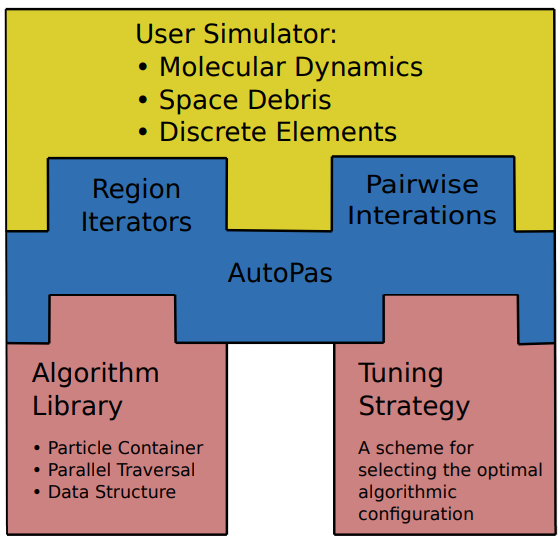
\includegraphics[width=2.2in]{figures/AutoPasLibraryStructure.png}
    \caption{AutoPas Library Structure as depicted by \cite{Newcome2023Poster}}
    \label{fig_architecture}
\end{figure}

\subsection{Algorithm Library}

All different algorithmic implementations for solving N-Body problems are part of the so called \textit{Algorithm Library} of AutoPas. The \textit{Algorithm Library} contains different implementations for certain key aspects of the simulation, such as neighbor identification, traversal patterns, and memory layouts.

Together they form a so called \textit{Configuration} fully describing the internal implementation of the engine. Such a configuration is a 6-tuple consisting of implementations for: \textit{Container}, \textit{Traversal}, \textit{Load Estimator}, \textit{Data Layout}, \textit{Newton 3}, and \textit{Cell Size Factor}.

An obvious benefit of this modular approach is the ability to easily swap out implementations for certain aspects of the simulation, without having to change the entire codebase. This allows for easy experimentation with different implementations and the ability to quickly adapt to new hardware or simulation scenarios.

Another benefit of this modular approach is presented with the ever growing configuration library of AutoPas. As the library is constantly updated and new implementations targeting specific hardware or simulation scenarios are added, it is possible to easily test the feasibility of older implementations
under new hardware \cite{Tchipev2020}.


\subsubsection{Container}

The \textit{Container} is responsible for storing the particles of the simulation such that relevant neighbor particles can be determinend efficiently. As AutoPas focuses on short-range interactions and uses a cutoff radius $r_c$, neighbor identification using just $O(N)$ distance calculations is possible \cite{Gratl2019AutoPas}. Such efficient neighbor identification are required for the simulation of large particle systems to be feasible. \autoref{fig_containers} shows the three most important container types used in AutoPas.

\begin{figure}[h]
    \centering
    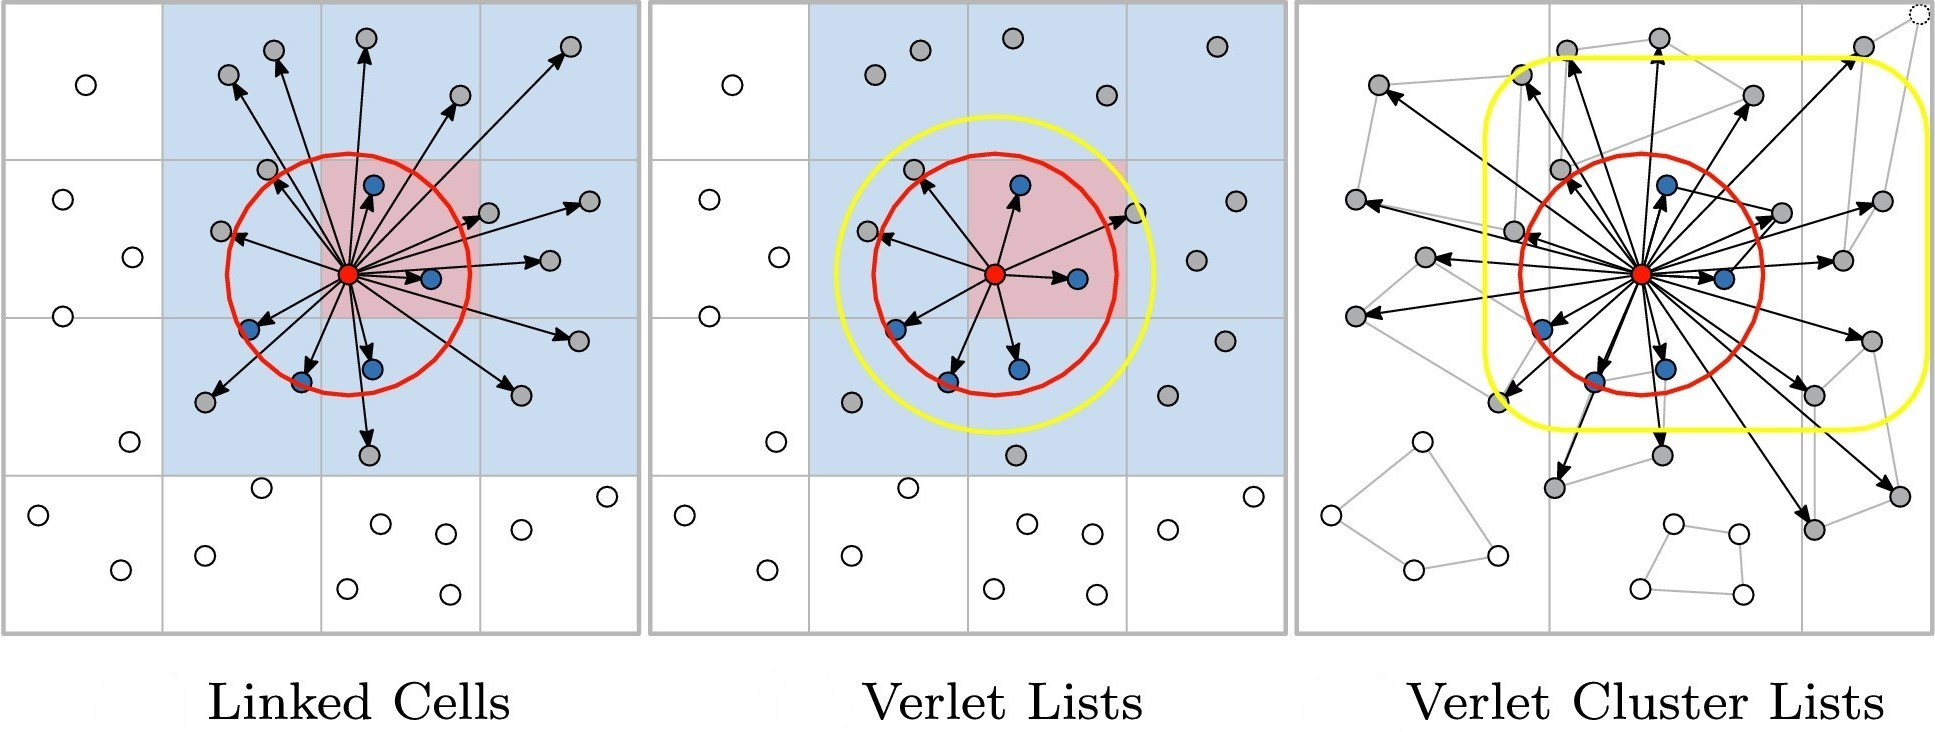
\includegraphics[width=\columnwidth]{figures/containers.jpg}
    \caption{Important Container Types as depicted by \cite{Gratl2022AutoPas}. The cut-off radius $\color{red} r_c$ is shown using a red circle.}
    \label{fig_containers}
\end{figure}


\begin{itemize}
    \item The \textit{LinkedCells} container maintains a grid of cells with a length of ${\color{red} r_c} * \textit{cellSizeFactor}$, where each cell contains a list of particles. When calculating the forces between particles, only neighboring cells (depicted as blue cells) need to be considered. All other particles are guaranteed to be outside the cut-off radius and can be ignored. \\
          LinkedCells typically come with a big overhead of useless distance calculations (shown by the many arrows in the figure), but are very cache friendly \cite{Gratl2022AutoPas}.

    \item The \textit{VerletList} container use a second radius $r_v = {\color{red} r_c} + \Delta_s$ (yellow circle) and considers all particles within this radius as potential neighbors. By introducing this buffer region, it is also possible to only rebuilt the neighbor-list every $N$ simulation steps, as long as no particle can move from outside $rc+ \Delta_s$ to inside $r_c$ unnoticed \cite{NEWCOME2023115278}. \\
          VerletLists can reduce the number of spurious distance calculations drastically, but cause far higher memory consumptions and are less cache friendly, reducing the vectorization potential \cite{Gratl2022AutoPas}.

    \item The \textit{Verlet Cluster Lists} container improves on the VerletList container by grouping particles into clusters of size $M$ ($M=4$ in the figures). When calculating the forces between particles, all particles from overlapping clusters within the $r_v$ radius need to be considered.\\
          Naturally this increases the number of spurious distance calculations again. However the number and size of the maintained lists can be reduced drastically. Furthermore $M$ can be chosen such that efficient vectorization is possible \cite{Gratl2022AutoPas}.

\end{itemize}


\subsubsection{Traversal}

\textit{Traversals} are responsible for iterating over the particles in the simulation and calculating the interactions between them in a shared-memory environment \cite{SECKLER2021101296}. The traversal pattern is a key aspect of the simulation engine, as it determines to which extent force calculations can be parallelized and wheter optimizations, such as Newton 3, can be applied.
By using Newton's third law, the number of force calculations can be reduced by half, as the force between two particles is equal and opposite. Not all traversal patterns support Newton 3, as it could introduce race conditions.



\todo{Traversal Types}


\subsubsection{Data Layout}

The \textit{Data Layout} is responsible for how the particle data is stored in memory. The choice of data layout can have a significant impact on the performance of the simulation engine, as it determines the memory access patterns and the potential for vectorization. Possible choices are \textit{SoA} (Structure of Arrays) and \textit{AoS} (Array of Structures). \textit{SoA} is typically more cache friendly and allows for better vectorization, however it causes information about a single particle to be spread across multiple memory locations. \textit{AoS} on the other hand stores all information about a single particle together, but prohibits efficient vectorization as filling vector registers requires gathering data from multiple memory locations.


\subsection{Auto-Tuning Framework}

Manually selecting the best implementations for each tunable parameter is a daunting task, and would require extensive domain knowledge difficult to acquire, and maintain under the constantly changing software and hardware landscape. To address this issue, AutoPas performs automated algorithm selection to maximize certain performance metrics, such as simulation speed or energy efficiency \cite{Gratl2022AutoPas}. The auto-tuning framework of AutoPas periodically initiates so called \textit{tuning-phases} in which it measures and evaluates promising\footnote{Promising configurations are suggested by so called TuningStragies} configurations in order to determine the best configuration for the current simulation state \cite{Gratl2019AutoPas}. The winning configuration is then used until the next tuning phase is initiated.

The key to efficient tuning phases is the ability to efficiently determine promising configurations. Just using the naive approach of evaluating all possible configurations turns out to be infeasible in practice, as many of the naively evaluated configurations turn out to be orders of magnitude slower than the best known configuration, thus causing a drastic increasing of the total simulation time \cite{endreport.pdf}\cite{Manuel_Lerchner_Thesis.pdf}.
As AutoPas is developed further, and new implementations are added to the algorithm portfolio, the number of possible configurations will steadily increase, further exacerbating the problem of naively evaluating all configurations.

AutoPas attempts to mitigate this problem by using so called \textit{TuningStrategies} which prune the search space of possible configurations based on certain criteria \cite{Gratl2019AutoPas}. A tuning strategy is tasked with the difficult job pruning enough configurations to make the tuning phase feasible, but not too many, as to not miss the optimal configuration. Tuning strategies need to balance the trade-off between potentially finding a better configuration and the cost of potentially encountering worse configurations during exploration \cite{Newcome2023Poster}.



\subsection{Static Optimization Techniques}

Static optimization techniques are primarily applied by compilers to generate efficient machine code for a given hardware architecture. As modern compilers are aimed at generating good average performance across a wide range of hardware platforms, default optimization settings are often not optimal for a specific hardware platform and application \cite{fursin2014collectivetuninginitiative}. To achieve optimal performance, some effort is required to tune the compiler settings to the specific hardware and application.

Another way to improve the performance of the generated code are profile-guided optimizations. Profile-guided optimizations use prior performance data collected during a simulation run to optimize the generated code for the specific workload during the next compilation.

Appart from the static optimization already performed by modern compilers, AutoPas is capable of performing basic tuning at compile time. As AutoPas hower primarily aims at dynamic optimization, the static optimization capabilities are limited to a set of compile-time flags that can be used to statically enable or disable certain features of the simulation engine, such as SIMD instructions, MPI support, or Auto-Vectorization \cite{Gratl2019AutoPas}. Those flags primarily aim at ensuring that the simulation engine can utilize the full potential of the hardware it is run on, but they are not used directly to tune the performance of the simulation engine.

\subsubsection{Kokkos Integration}

There are however attempts to expand the static optimization capabilities of AutoPas beyond just compile-time flags. One such attempt is the integration of the Kokkos library into AutoPas aiming to provide performance portability across different hardware platforms, and be able to run existing algorithms on GPGPUs \cite{Gärtner_KokkosInAutoPas.pdf}.

Kokkos is a performance-portable parallel programming model supporting diverse high-performance computing environments \cite{CARTEREDWARDS20143202}. Kokkos provides high-level C++ abstractions for parallel execution and memory management, enabling developers to write performance-portable code that can be compiled for different hardware architectures, including GPUs, Intel Xeon Phis, or many-core CPUs \cite{lammps_kokkos}.

The integration is still in an experimental phase and not yet capable of targeting systems other than conventional multi-core CPUs \cite{Gärtner_KokkosInAutoPas.pdf}.

A full integration of Kokkos into AutoPas could be beneficial as classical MD Simulation engines such as LAMMPS have demonstrated performance benefits from using Kokkos, particularly on large simulations on GPUs \cite{lammps_kokkos}. Supporting various hardware platforms could further demonstrate the usefulness of the AutoPas framework, as the performance of the algorithm library is highly dependent on the underlying hardware \cite{SECKLER2021101296} and changes in the optimal configuration are expected.

\section{Demonstration of Benefits of AutoTuning}

Even though AutoPas is designed to perform periodic auto-tuning, it often sufficient to just perform a single tuning phase at the beginning of the simulation, as many scenarios tend to behave fairly stable over time.
Simulating an inhomogeneous scenario can sometimes benefit from re-tuning the configuration after a number of simulation steps, especially when using a MPI environment with multiple nodes. Inhomogeneous scenarios can cause the load to be distributed unevenly both across the nodes and across time steps, further increasing the potential benefits of periodically re-tuning the configuration on each node.

The currently provided example runs from \texttt{md-flexible} are not sufficient to demonstrate the benefits of periodic re-tuning \todo{cite data from ba}. More complex scenarios, most likely involving multiple nodes and a high number of particles, are required to demonstrate the benefits of periodic re-tuning.

\newpage
\newpage


\section{Early Stopping Optimization}

As identified by \cite{autopas_issue673}\cite{endreport.pdf}\cite{Manuel_Lerchner_Thesis.pdf}, overhead caused by evaluating subobtimal configurations during the tuning phase can be a significant bottleneck in the performance of the AutoPas framework. Even though the tuning strategies employed by AutoPas are highly efficient, they still tend to suggest a large number of configurations that are not optimal. Rule driven tuning strategies such as \textit{RuleBasedTuning} and \textit{FuzzyTuning} can mitigate this problem to some extent, but due to the complexity of particle simulations, those rule-bases are expected to be highly incomplete.

All mentioned sources suggest that some form of \textit{early stopping} mechanism could be beneficial for the AutoPas framework. The primarily goal of such a mechanism would be to detect tuning-iterations that take much longer than the currently best known configuration and stop the evaluation of those configurations early. There are two approaches to this problem:

\begin{itemize}
    \item \textbf{Stopping Further Samples:} Currently AutoPas supports testing a certain parameter configuration multiple times to get a more accurate and stable performance measurement. A simple way to implement early stopping would be to stop the evaluation of further samples of a configuration if the performance of a sample is significantly worse than the best known configuration. The implementation of this approach would be relatively simple, but it is fairly course grained as all started samples would still be evaluated fully.
    \item \textbf{Interrupting the Evaluation:} A more fine grained approach as proposed in \cite{endreport.pdf} would be to interrupt the evaluation of a configuration as soon as it is clear that the performance is significantly worse than the best known configuration. This is way more difficult to implement, as it would require the ability to interrupt the evaluation of a configuration at any point in time. Especially in a MPI environment with multiple nodes, aborting and resetting the simulation to a consistent state would require a lot of synchronization and communication work.
\end{itemize}

Both mentioned approaches require a user defined threshold for the maximum allowed slowdown of a configuration before it should be stopped. This threshold will be determined empirically in \autoref{sec:evaluation}.

To get a first impression of the potential benefits of an early stopping mechanism, we implemented the first approach in the AutoPas framework. The changes to the existing codebase are minimal and the early stopping mechanism can be implemented using existing functionality. \autoref{alg_early_stopping} shows the implementation of the early stopping mechanism in the AutoPas framework.

\subsection{Implementation}
The early stopping mechanism is triggered by the new \texttt{CheckEarlyStopping} function, which is called after the performance of a configuration has been measured. The function compares the performance of the current configuration to the best known performance encountered in the current tuning phase. If the performance of the current configuration is significantly worse than the best known performance, the \texttt{abort} flag is set to \texttt{true}. The existing \texttt{GetNextConfiguration} function is modified slightky to trigger a re-tuning of the configuration if the \texttt{abort} flag is set. The \texttt{abort} flag is reset during re-tuning.



\begin{algorithm}[H]
    \small
    \caption{Early Stopping Algorithm in AutoPas}
    \label{alg_early_stopping}
    \begin{algorithmic}[1]
        \Procedure{CheckEarlyStopping}{performance}
        \State $fastestTime \gets \min(fastestTime, performance)$
        \State $slowdownFactor \gets \frac{performance}{fastestTime}$
        \If{$slowdownFactor > maxAllowedSlowdown$}
        \State $abort \gets true$
        \EndIf
        \EndProcedure

        \vspace{0.5em}

        \Procedure{GetNextConfiguration}{}
        \If{not $inTuningPhase$}
        \State \Return ($currentConfig, false)$
            \ElsIf{$numSamples$ $<$ $maxSamples$ \redbox{\textbf{and} not $abort$}}
            \State \Return $(currentConfig, true)$
            \Else
            \State $stillTuning \gets \Call{tuneConfiguration}{~}$
            \State \Return $(newConfig, stillTuning)$
        \EndIf
        \EndProcedure
    \end{algorithmic}

\end{algorithm}



\subsection{Evaluation}
\label{sec:evaluation}

This section evaluates the performance of the early stopping mechanism described in \autoref{alg_early_stopping}. The performance of the early stopping mechanism is evaluated for different values of the maximum allowed slowdown factor, in order to determine the optimal threshold for the early stopping mechanism.

All benchmarks are performed on the CoolMUC2 supercomputer \todo{reference} and are repeated 3 times to account for statistical variance.

\subsubsection{Exploding Liquid Simulation [Predictive Tuning]}

The first benchmark is performed with the \textit{Exploding Liquid} scenario present in the \texttt{md-flexible} framework. The simulation consists of 1764 initially close-packed particles that are simulated with a Lennard-Jones potential. During the simulation, the particles rapidly expand outwards and eventually hitting the simulation boundaries. The simulation is run with a single thread on a single node of the CoolMUC2 supercomputer.

\begin{figure}[H]
    \centering

    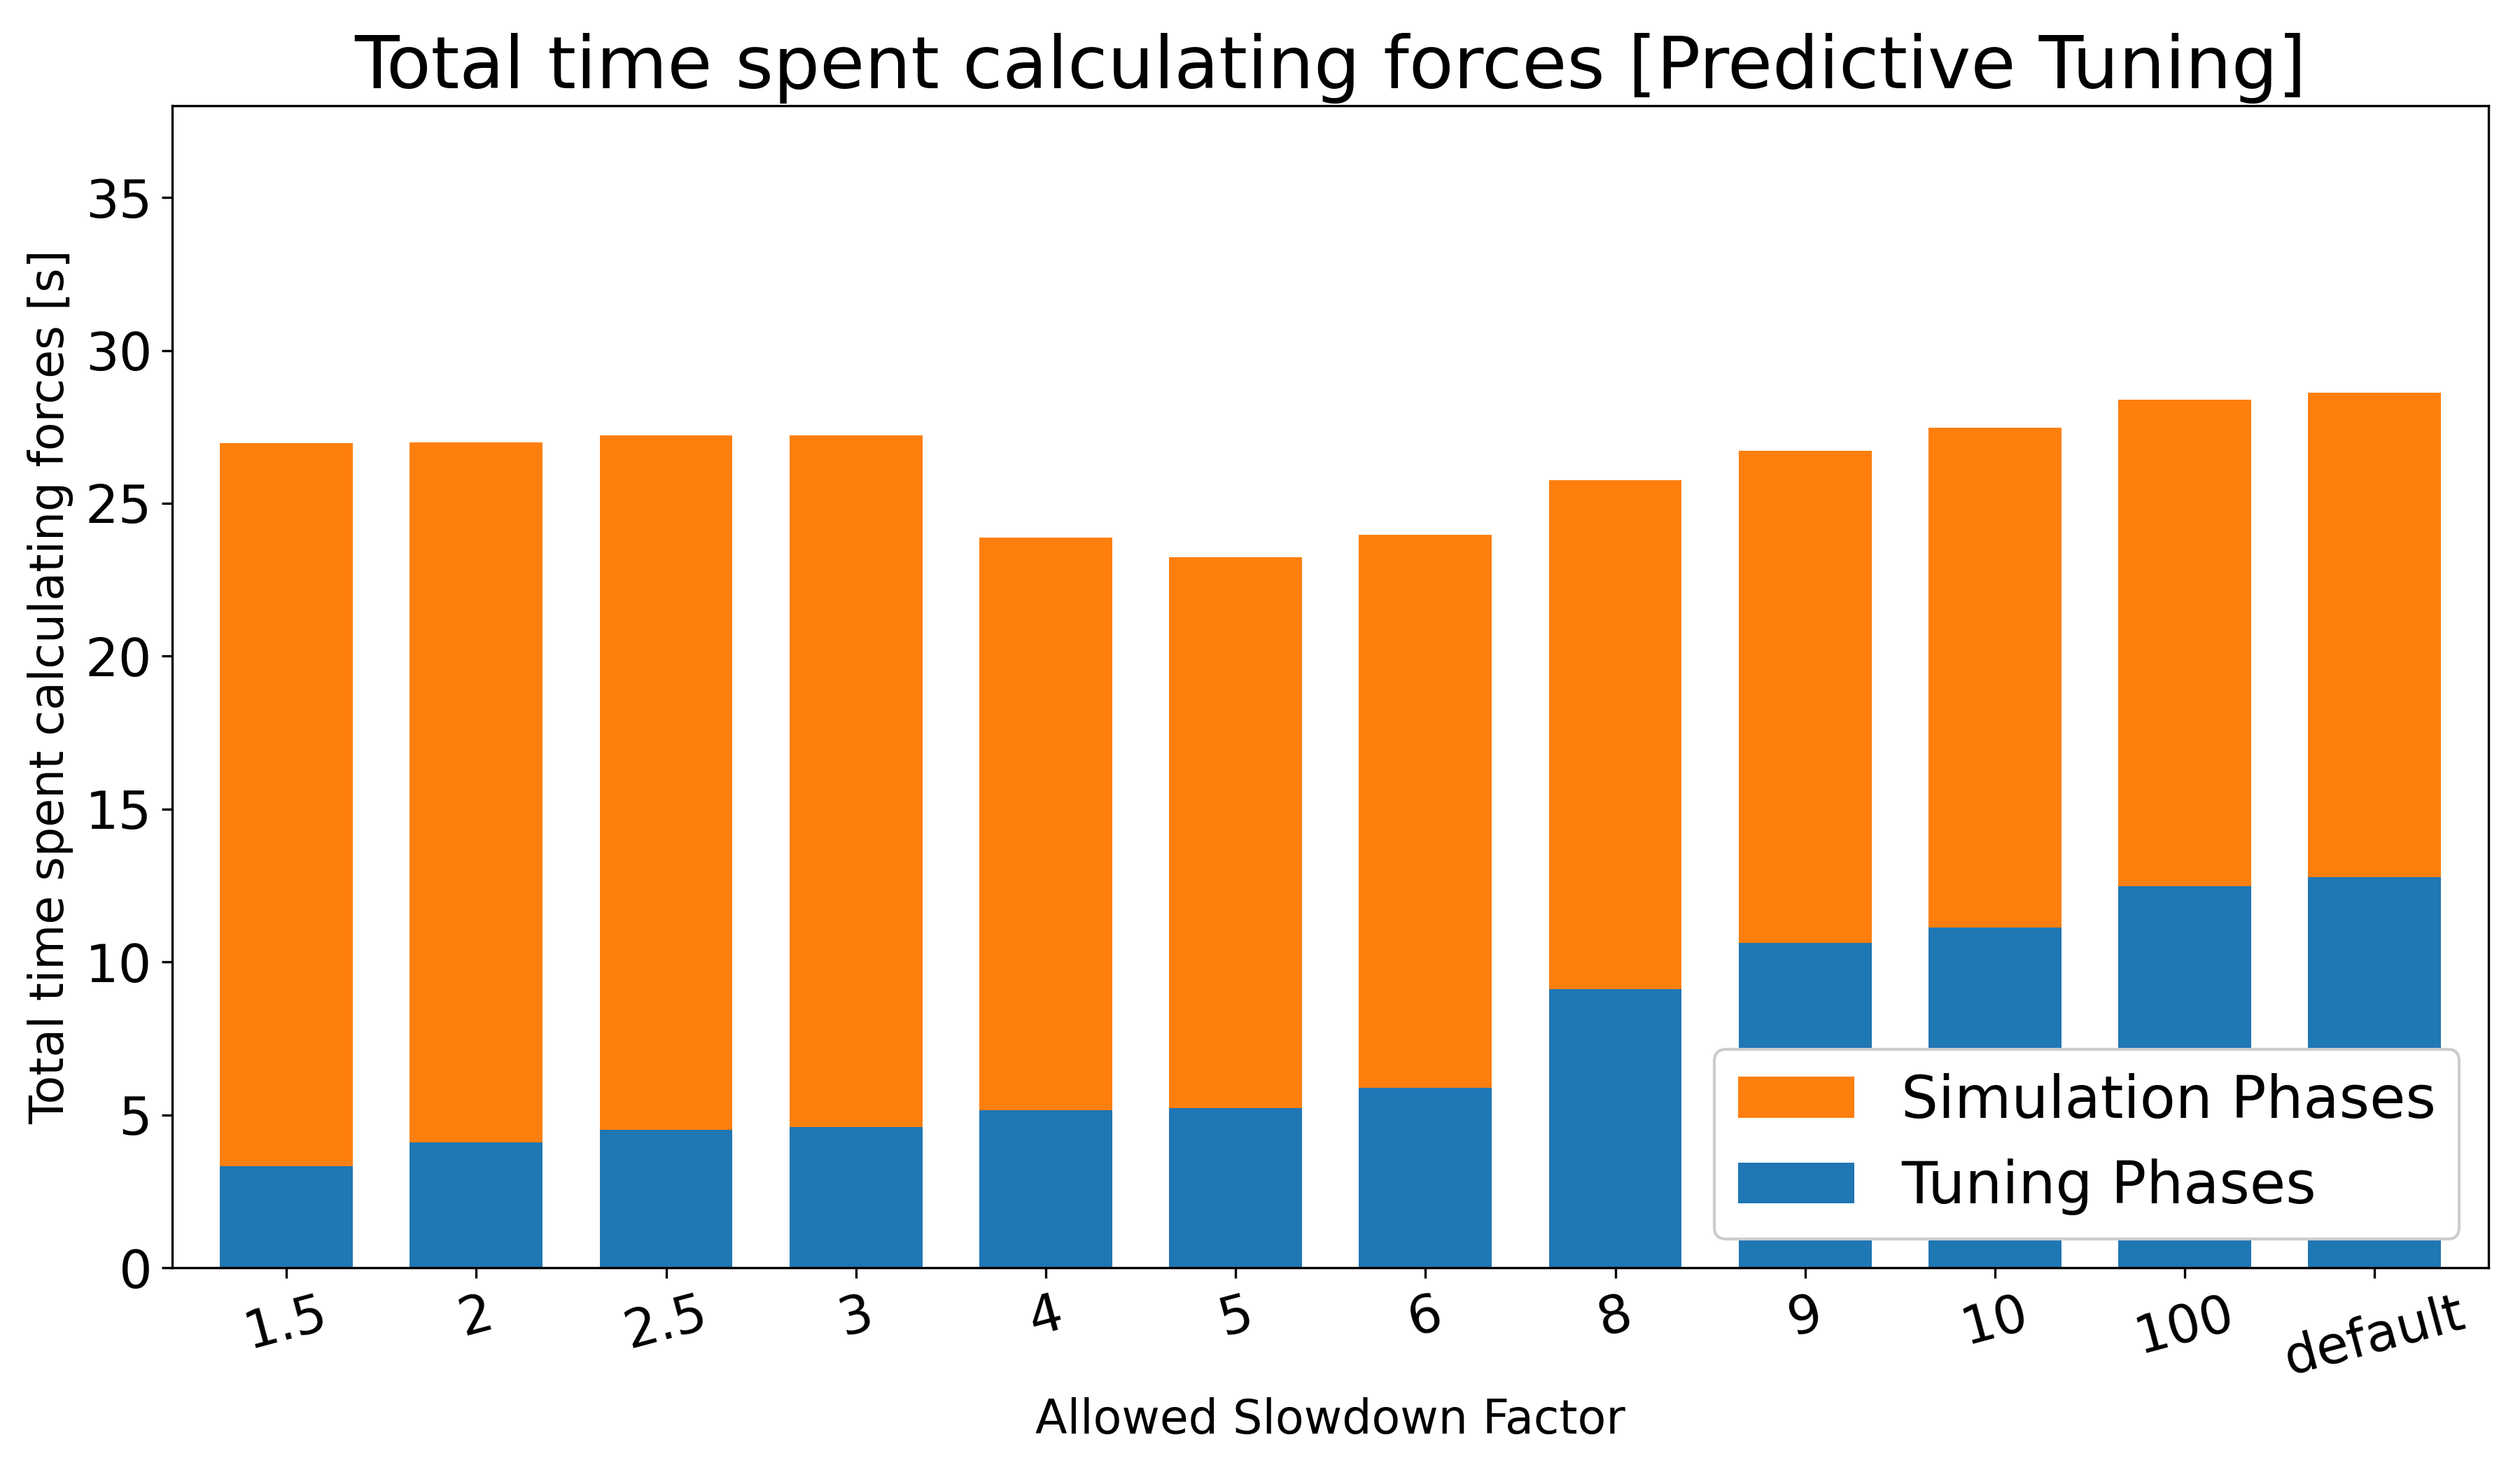
\includegraphics[width=\columnwidth]{../data/explodingLiquid/cluster/predictiveTuning/analytics/total_time_average.png}

    \caption{Total Simulation Time for Exploding Liquid Simulation with Early Stopping divided in tuning and simulation phases. The total simulation time is minimal at a maximum allowed slowdown factor of $\approx5$.}
\end{figure}

Compared to Predictive Tuning without early stopping, the early stopping mechanism can reduce the total simulation time from 28.62 seconds to 23.23 seconds when using a maximum allowed slowdown factor of 5. This is a reduction of 18.9\% in the total simulation time. The optimal threshold for the early stopping mechanism is around 5 for the \textit{Exploding Liquid} scenario.


\subsubsection{Exploding Liquid Simulation [Full Search]}


\subsection{Analysis and Discussion}

All evaluated benchmarks show that there exists just a slim range of optimal thresholds for the early stopping mechanism which actually reduce the total simulation time. This is expected, the two corner cases $maxAllowedSlowdown \to 1$ and $maxAllowedSlowdown \to \infty$ are expected to perform poorly. $maxAllowedSlowdown \to 1$ essentially results in tuning phases with just one sample per configuration, which is not enough to get a good estimate of the performance of a configuration and causes simulation phases with suboptimal configurations. On the other hand, $maxAllowedSlowdown \to \infty$ results in the early stopping mechanism never aborting a configuration, which is equivalent to always evaluating all samples of a configuration, even if the configuration is known to be suboptimal.

Consequently, the optimal threshold for the early stopping mechanism is a trade-off between the overhead of evaluating suboptimal configurations and the risk of missing optimal configurations due to noise in the performance measurements.

From the executed benchmarks, we deduce that the optimal threshold for the early stopping mechanism is around \todo{X} for the \textit{Exploding Liquid} scenario and around \todo{Y} for the \textit{Spinodal Decomposition} scenario, but it is expected that the optimal threshold is highly dependent on the specific simulation scenario and the environment the simulation is run in.

It is howerver noteworthy that the early stopping mechanism never caused a significant slowdown of the simulation, even if poor thresholds were chosen.

We conclude that the (naive) early stopping mechanism is a valuable addition to the AutoPas framework, as it can reduce the total simulation time significantly without causing any significant slowdowns.

\subsection{Future Work}

As the current implementation is only capable of stopping further samples of a configuration, the next step would be to extend the early stopping mechanism to dynamically blacklist certain implementations.

A crude way to implement this would be to create a set of parameters most influential to the performance of the simulation (for example: \{\textit{Particle Container}, \textit{Data Layout}\}) and blacklist configurations that use a certain values if there is enough evidence that a configuration with those values is not a good choice for the current simulation scenario (potentialy if more than $X$\% of samples using certain values are stopped early).

The parameter \textit{Particle Container} should be included in the set of parameters to blacklist, as it is known to be highly influential to the performance of the simulation \cite{Gratl2019AutoPas}.


\newpage
\newpage


\section{State of the Art in MD Simulations}


\subsection{GROMACS}

\subsubsection{Static Optimization Techniques}


\subsubsection{Dynamic Optimization Strategies}




\subsection{LAMMPS}

\subsubsection{Static Optimization Techniques}


\subsubsection{Dynamic Optimization Strategies}



\subsection{Feature Comparison of MD Engines}


% Include a comparison table
\begin{table}[H]
    \caption{Feature Comparison of MD Engines}
    \label{table_comparison}
    \centering
    \begin{tabular}{|l|c|c|c|}
        \hline
        \textbf{Feature}       & \textbf{AutoPas} & \textbf{GROMACS} & \textbf{LAMMPS} \\
        \hline
        Auto-tuning            & \checkmark       & Partial          & Partial         \\
        \hline
        GPU Support            & \checkmark       & \checkmark       & \checkmark      \\
        \hline
        Dynamic Load Balancing & \checkmark       & \checkmark       & \checkmark      \\
        \hline
    \end{tabular}
\end{table}


\subsection*{Limitations of those Approaches}

As mentioned earlier, both GROMACS and LAMMPS focus primarily on static optimization. While these techniques are heavily optimized, both engines are not capable of performing datastructure and algorithm changes at runtime. This limitation can lead to suboptimal performance in situations where the chosen implementation is not optimal. Those situations can also arise during the simulation, when the simulation state changes such that other datastructures or algorithms would be more efficient.




\subsection{Performance Comparison}


Different engines excel in various scenarios:
\begin{itemize}
    \item Large-scale simulations
    \item GPU-accelerated computations
    \item Memory-constrained environments
\end{itemize}



\begin{itemize}
    \item AutoPas demonstrates superior performance in various scenarios.
    \item GROMACS and LAMMPS show competitive performance in specific use cases.
    \item Auto-tuning plays a crucial role in optimizing performance across different engines.
\end{itemize}



\section{Conclusion}

\subsection{Summary of Findings}

This study provides a comprehensive comparison of auto-tuning approaches in modern MD engines, highlighting the unique advantages of AutoPas's implementation while acknowledging the strengths of established frameworks like GROMACS and LAMMPS.

\subsection{Future Directions}

Future research directions include:
\begin{itemize}
    \item Further optimization of auto-tuning strategies
    \item Integration of machine learning techniques for performance prediction
    \item Collaboration between MD engine developers to share optimization strategies
\end{itemize}

\cite{Gratl2019AutoPasAF}


\bibliographystyle{IEEEtran}
\bibliography{literature}



\newpage
\newpage
\tableofcontents

\end{document}

